\documentclass[10.5pt,fontset=fandol]{ctexart}
\usepackage[paperwidth=222.6413mm,paperheight=297mm,left=1.9cm,right=1.9cm,top=2.1cm,bottom=1.8cm,headsep=0.5cm]{geometry}
\usepackage{amsmath,amssymb,mathrsfs}
\usepackage[table]{xcolor}
\usepackage{booktabs,tabularx,xltabular,needspace,array,ragged2e,enumitem,tcolorbox,tikz,fancyhdr}
\tcbuselibrary{skins,breakable}
\usepackage[hidelinks]{hyperref}
\definecolor{deepblue}{HTML}{1B3A5C}\definecolor{navy}{HTML}{1B3A5C}\definecolor{accentred}{HTML}{B23A48}\definecolor{accentA}{HTML}{B23A48}
\definecolor{muted}{HTML}{5A6470}\definecolor{qbg}{HTML}{F4F6F8}\definecolor{linec}{HTML}{9AA3AD}
\newcolumntype{L}[1]{>{\RaggedRight\arraybackslash}p{#1}}
\newlist{qp}{enumerate}{1}\setlist[qp]{label=(\alph*),leftmargin=1.5em,itemsep=2pt}
\newlist{qn}{enumerate}{1}\setlist[qn]{label=(\arabic*),leftmargin=1.5em,itemsep=2pt}
\newlist{qparts}{enumerate}{1}\setlist[qparts]{label=(\alph*),leftmargin=1.5em,itemsep=2pt}
\newlist{qnum}{enumerate}{1}\setlist[qnum]{label=(\arabic*),leftmargin=1.5em,itemsep=2pt}
\newlist{bul}{itemize}{1}\setlist[bul]{label=\textbullet,leftmargin=1.5em,itemsep=2pt}
\newcommand{\key}[1]{\par\vspace{4pt}\noindent\textbf{\color{navy}#1}\par\vspace{2pt}}
\newcommand{\hint}[1]{\par\smallskip{\small\itshape Hint: #1}\par}
\newcommand{\sect}[1]{{\small\color{muted}#1}}
\newcommand{\dd}{\mathrm d}\newcommand{\Var}{\operatorname{Var}}\newcommand{\Cov}{\operatorname{Cov}}
\newcommand{\E}{\mathbb E}\newcommand{\ee}{\mathrm e}\newcommand{\jj}{\mathrm j}
\newtcolorbox{workspace}{height fill,enhanced,colback=white,colframe=linec!55,boxrule=0.5pt,arc=1.5pt}
\newcommand{\qtitle}[2]{\par\addvspace{.85em}\Needspace{10\baselineskip}\begin{tcolorbox}[colback=navy,colframe=navy,arc=1.5pt,boxrule=0pt]\color{white}\large\bfseries #1\hfill\small #2\end{tcolorbox}}
\pagestyle{fancy}\fancyhf{}\fancyhead[L]{\footnotesize\color{navy}SSA -- Chapter 3 -- Solutions}\fancyhead[R]{\footnotesize\thepage}
\fancyfoot[C]{\scriptsize Eight-paper edition -- 2026-10-27}
\newcommand{\step}[1]{\par\addvspace{.4em}\Needspace{4\baselineskip}\textbf{#1}\par}\hypersetup{pdftitle={SSA Chapter 3 Review Solutions - Chinese}}


\begin{document}

\begin{titlepage}\centering\vspace*{1.5cm}{\Huge\bfseries 随机信号分析}\par\vspace{1cm}{\LARGE\bfseries 第3章复习习题集中文详解}\par\vspace{6mm}{\large 平稳性与功率谱密度}\par\vspace{1cm}{\large 21题 · 7天 · 每天3题}\par\vspace{1cm}

\begin{tcolorbox}[colback=qbg,colframe=navy]与英文题集逐题对应，全部10道作业题均完整解答。按连续阅读排版，保留推导、条件与特殊边界，不添加手写留白。\par 八套真题的本章核心均值为13.25分/套，近期四套为19.50分/套。对原卷或教材中不适用于普通有限方差过程的表达，分别说明可确定结论、广义函数解释和显式改编。\end{tcolorbox}\vfill 2026年10月27日\end{titlepage}

\section*{题号、来源与教材小节}

{\small\renewcommand{\arraystretch}{1.15}\begin{xltabular}{\textwidth}{@{}r r L{9.4cm} X@{}}\toprule 题 & 天 & 来源 & 教材小节\\\midrule\endfirsthead\toprule 题 & 天 & 来源 & 教材小节\\\midrule\endhead\midrule\multicolumn{4}{r}{\small 索引续下页}\\\endfoot\bottomrule\endlastfoot

1 & 1 & Original recall and counterexample & 3.1.1\\

2 & 1 & Textbook 3.1 / Optional homework & 3.1.1\\

3 & 1 & Textbook 3.4 / Required homework & 3.1.1\\

4 & 2 & Textbook 3.5 / Required homework & 3.1.1 / 3.3.1\\

5 & 2 & Textbook 3.9 / Required homework & 3.1.2 / 3.3.1\\

6 & 2 & Adapted from 202312 Q1; finite-power correction & 3.1.1 / 3.1.2 / 3.4.2\\

7 & 3 & Adapted from 202112 Q2(a--d) & 3.1.1 / 3.1.2 / 3.3.1\\

8 & 3 & Textbook 3.7 / Optional homework & 3.2.2\\

9 & 3 & Textbook 3.14 / Required homework & 3.3.1 / 3.4.2\\

10 & 4 & Textbook 3.16 / Required homework & 3.1.1 / 3.3.1\\

11 & 4 & Textbook 3.21 / Required homework & 3.4.2\\

12 & 4 & Original transform-pair exercise & 3.3.1 / 3.3.2 / 3.4.2\\

13 & 5 & Textbook 3.25 / Required homework & 3.4.2\\

14 & 5 & Textbook 3.19 / Optional homework & 3.4.2\\

15 & 5 & Adapted from 202212 Q2(a--c) & 3.1.1 / 3.4.2\\

16 & 6 & Adapted from 202512 Q2(a,b); consistent amplitude model & 3.1.1 / 3.4.2\\

17 & 6 & Adapted from 202412 Q2(a,b); zero means and nonzero carrier specified & 3.1.1 / 3.1.2 / 3.4.2\\

18 & 6 & Adapted from 202412 Q1(a--c) & 3.1.1 / 3.1.2\\

19 & 7 & Adapted from 202112 Q4(a); carrier separation stated & 3.3.2 / 3.4.2\\

20 & 7 & Original exercise; tools used in 202104 Q2 and recent RC-noise questions & 3.3.2 / 3.4.2 / 3.5.1\\

21 & 7 & Original diagnostic based on 202312 Q1 and 202512 Q2(c) & 3.1.1 / 3.3.2 / 3.4.2\\

\end{xltabular}}

\par\medskip 统一采用$R_{XY}(\tau)=\E[X(t+\tau)Y(t)]$，傅里叶正变换核为$e^{-j\omega\tau}$，反变换系数为$1/(2\pi)$。题源标签中的改编条件是复习题显式添加的条件。\clearpage

\qtitle{解答 1：平稳定义与反例}{第1天}
{\small\color{accentred}Original recall and counterexample}\par{\small\color{muted}教材小节：3.1.1}\par\smallskip\step{1. 先区分分布不变与二阶特征不变。}
严格平稳要求：任意$n$、任意$t_1,\ldots,t_n$和共同平移$u$，向量$(X(t_i))_{i=1}^n$与$(X(t_i+u))_{i=1}^n$同分布。广义平稳要求二阶矩有限、$m_X(t)=m$为常数，且$R_X(t+\tau,t)=R_X(\tau)$只依赖时差。
严格平稳的一维分布不变，所以均值不变；二维分布在共同平移下不变，所以有限的二阶矩只依赖时差。因此严格平稳加有限二阶矩推出广义平稳。若没有二阶矩，不能作此推断。
\step{2. 高斯过程为什么是例外。}
任意有限维向量都联合高斯时，其分布由均值向量和协方差矩阵确定。WSS使均值向量的各分量均为$m$，协方差矩阵元素为$C_X(t_i-t_j)$；共同平移不改变两者，因此所有有限维分布不变，即SSS。仅有各时刻边缘高斯不够，必须是联合高斯过程。
\step{3. 用一个连续样本的反例否定一般逆命题。}
令$A,B$为独立公平符号（等概率$\pm1$），$X(t)=A\cos t+B\sin t$。由$\E A=\E B=\E AB=0$及$\E A^2=\E B^2=1$，
\[m_X(t)=0,\qquad R_X(s,t)=\cos s\cos t+\sin s\sin t=\cos(s-t).\]
故它WSS。但$X(0)=A$只取$\pm1$，而$X(\pi/4)=(A+B)/\sqrt2$取$-\sqrt2,0,\sqrt2$，概率为$1/4,1/2,1/4$。一维分布已随时间变化，所以不是SSS。

\qtitle{解答 2：独立采样过程}{第1天}
{\small\color{accentred}Textbook 3.1 / Optional homework}\par{\small\color{muted}教材小节：3.1.1}\par\smallskip\step{1. 不同时刻使用独立性。}
每个时刻$U(t)\sim N(0,2)$，因此
\[f(u;t)=\frac1{2\sqrt\pi}e^{-u^2/4}.\]
若$t_1\ne t_2$，联合密度是两个一维密度的乘积：
\[f(u_1,u_2;t_1,t_2)=\frac1{4\pi}e^{-(u_1^2+u_2^2)/4}.\]
对于两两不同的$t_1,\ldots,t_k$，
\[\boxed{f(\boldsymbol u;\boldsymbol t)=(4\pi)^{-k/2}\exp\left(-\frac14\sum_{i=1}^ku_i^2\right)}.\]
\step{2. 重复时刻不是独立的新抽样。}
若$t_1=t_2$，两个坐标相等，普通二维密度不存在；可写广义密度$f(u_1;t_1)\delta(u_2-u_1)$。一般情形先把相同时间归为一组，只对各组代表变量的独立密度相乘，并在组内加入相等的支撑约束。
共同时间平移不改变任何两时刻是否相等，全部有限维分布不变，故严格平稳。又
\[m_U=0,\qquad R_U(\tau)=\begin{cases}2,&\tau=0,\\0,&\tau\ne0,\end{cases}\]
二阶矩有限，故也广义平稳。这里的相关不是$2\delta(\tau)$：一个在单点取有限值的函数，与Dirac广义函数不同。该连续参数独立抽样模型不具均方连续性；不能直接当作具有普通样本函数的理想连续时间白噪声。

\qtitle{解答 3：独立平稳过程的乘积}{第1天}
{\small\color{accentred}Textbook 3.4 / Required homework}\par{\small\color{muted}教材小节：3.1.1}\par\smallskip\step{1. 广义平稳的证明。}
题目的独立应理解为两个过程整体独立，涵盖任意有限维采样向量；仅有每个同时刻$X(t)$与$Y(t)$独立不能保证下面的跨时刻分解。
\[m_Z=\E[XY]=m_Xm_Y,\]
\[\begin{aligned}R_Z(t+\tau,t)&=\E[X(t+\tau)X(t)Y(t+\tau)Y(t)]\\&=R_X(\tau)R_Y(\tau).\end{aligned}\]
均值为常数、相关只依赖时差；$\E Z^2=\E X^2\E Y^2<\infty$，所以$Z$为WSS。
\step{2. 若“平稳”指严格平稳。}
分别取向量$\boldsymbol X=(X(t_i))$、$\boldsymbol Y=(Y(t_i))$。独立性使联合律为两者分布的乘积；共同平移保持两个分布不变，故保持联合律不变。再作确定映射$(\boldsymbol x,\boldsymbol y)\mapsto(x_iy_i)_i$，得到的$Z$向量分布也不变。此证明不要求存在密度，也不需要额外矩条件。

\qtitle{解答 4：平方律器件输出}{第2天}
{\small\color{accentred}Textbook 3.5 / Required homework}\par{\small\color{muted}教材小节：3.1.1 / 3.3.1}\par\smallskip\step{1. 把平方写成直流项加二倍频。}
\[Y(t)=100\sin^2(\omega_0t+\Theta)=50-50\cos(2\omega_0t+2\Theta).\]
相位均匀使余弦平均为0，所以$\boxed{m_Y=50}$。
\step{2. 同一相位在两个样本中保留后再取平均。}
用$\cos a\cos b=[\cos(a-b)+\cos(a+b)]/2$；和角项含$4\Theta$，其期望为0，而差角为$2\omega_0\tau$。因此
\[\boxed{R_Y(\tau)=2500+1250\cos(2\omega_0\tau)}.\]
均值恒定且相关只依赖$\tau$，所以WSS。进一步
\[\E Y^2=3750,\quad \Var(Y)=1250,\quad C_Y(\tau)=1250\cos(2\omega_0\tau).\]
即使$\omega_0=0$也成立，此时每条样本函数为随试验改变的时间常量。

\qtitle{解答 5：和差与互相关}{第2天}
{\small\color{accentred}Textbook 3.9 / Required homework}\par{\small\color{muted}教材小节：3.1.2 / 3.3.1}\par\smallskip\step{1. 展开前确认交叉项。}
由于过程独立且均值都为0，对任意$s,t$有$\E[X(s)Y(t)]=0$。按$R_{ZW}(\tau)=\E[Z(t+\tau)W(t)]$，
\[\begin{aligned}
R_Z&=R_X+R_Y+R_{XY}+R_{YX},\\
R_W&=R_X+R_Y-R_{XY}-R_{YX},\\
R_{ZW}&=R_X-R_Y-R_{XY}+R_{YX}.
\end{aligned}\]
故
\[\boxed{R_Z(\tau)=R_W(\tau)=e^{-|\tau|}+\cos(2\pi\tau)},\]
\[\boxed{R_{ZW}(\tau)=e^{-|\tau|}-\cos(2\pi\tau)}.\]
$R_Z(0)=R_W(0)=2$，$R_{ZW}(0)=0$。后者只说明同时刻不相关，不能自动推出$Z,W$独立。

\qtitle{解答 6：联合平稳与有理谱}{第2天}
{\small\color{accentred}Adapted from 202312 Q1; finite-power correction}\par{\small\color{muted}教材小节：3.1.1 / 3.1.2 / 3.4.2}\par\smallskip\step{1. 联合平稳与线性组合。}
独立的零均值WSS过程有$R_{XY}(s,t)=0$，两个自相关只依赖时差，故$X,Y$联合WSS。它们的任意确定线性组合也具有常均值、时差型的全部自/互相关，所以$Z,V$联合WSS。
\step{2. 先反变换两个给定谱。}
利用$e^{-a|\tau|}\leftrightarrow2a/(a^2+\omega^2)$，
\[R_X(\tau)=2e^{-4|\tau|},\qquad R_Y(\tau)=2e^{-2|\tau|}.\]
于是
\[\boxed{S_Z(\omega)=\frac{16}{\omega^2+16}+\frac8{\omega^2+4}},\]
\[\boxed{R_{XZ}(\tau)=2e^{-4|\tau|}},\qquad
\boxed{R_{VZ}(\tau)=2e^{-4|\tau|}-2e^{-2|\tau|}}.\]
采用“第一个过程取$t+\tau$”的约定。该题明确用有限功率谱替换了原卷的$\omega^2/(\omega^2+16)$；此替换是复习题的修改，并非原题照录。原谱的广义解释见解答21。

\qtitle{解答 7：带时延的雷达回波}{第3天}
{\small\color{accentred}Adapted from 202112 Q2(a--d)}\par{\small\color{muted}教材小节：3.1.1 / 3.1.2 / 3.3.1}\par\smallskip\step{1. 同时平移两个输入时刻。}
$\E Y=0$。展开两个$Y$样本的乘积，独立零均值使所有$X,N$交叉项消失，得到
\[\boxed{R_Y(\tau)=\alpha^2R_X(\tau)+R_N(\tau)}.\]
$Y$均值不变、相关为时差函数，且二阶矩有限，所以WSS。
\step{2. 时延符号来自明确的时间差。}
\[\begin{aligned}R_{XY}(\tau)&=\E[X(t+\tau)Y(t)]
=\alpha\E[X(t+\tau)X(t-d)]\\&=\boxed{\alpha R_X(\tau+d)},\\
R_{YX}(\tau)&=\E[Y(t+\tau)X(t)]
=\boxed{\alpha R_X(\tau-d)}.
\end{aligned}\]
第一个过程的时间减去第二个过程的时间分别为$\tau+d$和$\tau-d$。实WSS过程的自相关为偶函数，因此两结果满足$R_{YX}(\tau)=R_{XY}(-\tau)$。它们都只依赖时差，连同两个自相关及恒定均值，证明$X,Y$联合WSS。

\qtitle{解答 8：循环平稳的周期平移}{第3天}
{\small\color{accentred}Textbook 3.7 / Optional homework}\par{\small\color{muted}教材小节：3.2.2}\par\smallskip\step{1. 循环平稳允许怎样平移。}
周期100意味着$m(t+100k)=m(t)$，以及
\[R(t_1+100k,t_2+100k)=R(t_1,t_2),\qquad k\in\mathbb Z.\]
相关函数的两个时间必须同时平移相同的整周期，不能分别随意平移。
\step{2. 对每个期望应用线性性。}
\[\begin{aligned}
\E[5Y(110)]&=5m(10)=\boxed{100},\\
\E[10Y(310)+50]&=10m(10)+50=\boxed{250},\\
\E[Y(105)Y(101)]&=R(5,1)=\boxed{10},\\
\E[30Y(205)Y(201)+200]&=30R(5,1)+200=\boxed{500},\\
\E[10Y(305)Y(301)+6Y(210)+80]&=10R(5,1)+6m(10)+80=\boxed{300}.
\end{aligned}\]
这里不需要不同时间样本独立，也不能把乘积的期望替换为均值的乘积。

\qtitle{解答 9：自相关函数的可行性}{第3天}
{\small\color{accentred}Textbook 3.14 / Required homework}\par{\small\color{muted}教材小节：3.3.1 / 3.4.2}\par\smallskip\step{1. 判别时同时检查方差与谱正性。}
实WSS自相关必须为实偶函数，$R(0)=\sigma^2+m^2$，并且正半定。非负且总质量有限的谱测度可以充分保证正半定性；仅有偶性与$|R(\tau)|\le R(0)$并不充分。
\begin{enumerate}
\item $5u(\tau)e^{-3\tau}$不是偶函数，拒绝；$u(0)$的约定不改变结论。
\item $5\sin5\tau$为奇函数且$R(0)=0\ne5$，拒绝。
\item $9/(1+2\tau^2)$本身可作某零均值过程的自相关，但$R(0)=9$，与指定$\sigma_Y^2=10$不符，故拒绝作为本题的$R_Y$。
\item $-\cos6\tau\,e^{-|\tau|}$在0处为$-1$，均方值不能为负，拒绝。
\end{enumerate}
\step{2. 对(5)--(8)给出充分的非负谱构造。}
令$\Lambda(x)=\max(1-|x|,0)$，相应谱为
\[\begin{aligned}
S_{(5)}&=\frac{5\pi}{3}\Lambda(\omega/6),\\
S_{(6)}&=12\pi\delta(\omega)+\frac{2\pi}{5}\mathbf1_{\{|\omega|<10\}},\\
S_{(7)}&=\frac{10}{1+\omega^2},\\
S_{(8)}&=12\pi\delta(\omega)+4\sqrt{\pi/3}\,e^{-\omega^2/12}.
\end{aligned}\]
它们均非负、总质量有限，逆变换恰为题给函数；(5)(7)的$R(0)=5$，(6)(8)的$R(0)=10$。所以$\boxed{(5),(6),(7),(8)\text{可行}}$。
后两者中的常数6可来自一个\textbf{零均值、方差6的随机时间常量}，并不迫使均值非零。这一点也说明不能未经附加条件使用$\lim_{|\tau|\to\infty}R(\tau)=m^2$。

\qtitle{解答 10：同一个随机幅度}{第4天}
{\small\color{accentred}Textbook 3.16 / Required homework}\par{\small\color{muted}教材小节：3.1.1 / 3.3.1}\par\smallskip\step{1. 先证明$m_X=0$。}
已知$|R_X(\tau)|\le2e^{-|\tau|}$，且相关连续，故可定义均方意义的时间平均$\overline X_T=T^{-1}\int_0^T X(t)dt$。由柯西不等式，
\[\begin{aligned}
m_X^2&=|\E\overline X_T|^2\le\E\overline X_T^2\\
&\le\frac1{T^2}\int_0^T\!\int_0^T2e^{-|t-s|}\,ds\,dt\le\frac4T.
\end{aligned}\]
令$T\to\infty$，得$m_X=0$；不需要另假设各态历经，也不必确定$m_Y$。
\step{2. 两个时刻用的是同一个$A$。}
\[\E A^2=9+2^2=13,\qquad \boxed{m_Z=\E A\,m_Xm_Y=0}.\]
\[\begin{aligned}R_Z(\tau)&=\E A^2\,R_X(\tau)R_Y(\tau)\\
&=\boxed{26e^{-|\tau|}\cos(\omega_0\tau)(9+e^{-3\tau^2})}.
\end{aligned}\]
最后$\boxed{\Var[Z(t)]=R_Z(0)=260}$。不能把$\E A^2$误写成$(\E A)^2$，因为$A$不是在每个时刻重新独立抽取的。

\qtitle{解答 11：实信号功率谱判别}{第4天}
{\small\color{accentred}Textbook 3.21 / Required homework}\par{\small\color{muted}教材小节：3.4.2}\par\smallskip\step{1. 实信号PSD的条件。}
普通有限功率实WSS信号的谱应为实、偶、非负、有限总质量的测度。谱为函数时须可积，含冲激时其质量须非负。
\begin{enumerate}
\item $[\sin\omega/\omega]^2$非负、偶、实，在0处取连续极限1，在无穷远为$O(\omega^{-2})$，可行。
\item 分母$\omega^6+3\omega^2+3$对实$\omega$恒正；整个函数非负、偶、实，在0处正常，在无穷远为$O(\omega^{-4})$，可积，可行。
\item 在$0<|\omega|<1$时普通部分已为负，还有$\pm1$处极点与负权冲激$-\delta(\omega)$，不可能为PSD。
\item 非零$\omega$时通常为复数，不能作实信号的自功率谱。
\item $|\omega|/(1+\omega^2)^2$非负、偶、实且可积。其积分为$2\int_0^\infty\omega/(1+\omega^2)^2d\omega=1$，对应功率$1/(2\pi)$，可行。
\item $e^{-(\omega-1)^2}$虽非负可积，却不关于0偶对称，不能作为实信号PSD；复信号不受此偶性限制。
\end{enumerate}
综上$\boxed{(1),(2),(5)\text{可行}}$。复互谱可有虚部，与实信号自功率谱的条件不能混淆。

\qtitle{解答 12：连续谱与离散谱线}{第4天}
{\small\color{accentred}Original transform-pair exercise}\par{\small\color{muted}教材小节：3.3.1 / 3.3.2 / 3.4.2}\par\smallskip\step{1. 对连续项与谱线分别变换。}
\[\boxed{S_X(\omega)=\frac{12}{9+\omega^2}
+4\pi[\delta(\omega-5)+\delta(\omega+5)]+2\pi\delta(\omega)}.\]
指数项用$e^{-a|\tau|}\leftrightarrow2a/(a^2+\omega^2)$，余弦对应一对谱线，常数1对应$2\pi\delta(\omega)$。代入$\tau=0$，
\[\boxed{P_X=R_X(0)=2+4+1=7}.\]
\step{2. 构造零均值过程说明直流谱线的来源。}
取三个相互独立的分量：零均值WSS过程$G(t)$，相关为$2e^{-3|\tau|}$；$C(t)=\sqrt8\cos(5t+\Theta)$，其中$\Theta$均匀相位，相关为$4\cos5\tau$；随机常量$B$等概率取$\pm1$，相关为1。令$X=G+C+B$即可。
$G$的存在可由非负可积谱$12/(9+\omega^2)$构造平稳高斯过程保证。每个分量均值都是0，独立性消除交叉项。$B$在每条样本中不随时间变化，但试验间可正可负，因此零均值与零频谱线并不矛盾。

\qtitle{解答 13：互相关与共轭互谱}{第5天}
{\small\color{accentred}Textbook 3.25 / Required homework}\par{\small\color{muted}教材小节：3.4.2}\par\smallskip\step{1. 固定互相关方向和傅里叶符号。}
\[R_{XY}(\tau)=\E[X(t+\tau)Y(t)],\qquad
S_{XY}(\omega)=\int R_{XY}(\tau)e^{-j\omega\tau}\,d\tau.\]
对给定函数直接积分，
\[S_{XY}(\omega)=9\int_0^\infty e^{-(3+j\omega)\tau}d\tau
=\boxed{\frac9{3+j\omega}}.\]
0处单个端点值不影响积分。实联合WSS过程满足$R_{YX}(\tau)=R_{XY}(-\tau)$，故
\[\boxed{S_{YX}(\omega)=S_{XY}^*(\omega)=\frac9{3-j\omega}}.\]
$S_{XY}$的实部为$27/(9+\omega^2)$，虚部为$-9\omega/(9+\omega^2)$。互谱可为复数且不要求非负。这里完成的是题给互相关的形式傅里叶变换；题目未给两个自谱，不能据此完成联合谱可实现性的检查。

\qtitle{解答 14：反变换与无限功率边界}{第5天}
{\small\color{accentred}Textbook 3.19 / Optional homework}\par{\small\color{muted}教材小节：3.4.2}\par\smallskip\step{1. 有理谱先作部分分式。}
\[\frac{\omega^2}{(\omega^2+1)(\omega^2+2)}
=-\frac1{\omega^2+1}+\frac2{\omega^2+2}.\]
利用指数相关的变换对，
\[\boxed{R_X(\tau)=-\frac12e^{-|\tau|}+\frac1{\sqrt2}e^{-\sqrt2|\tau|}},
\qquad\boxed{\E X^2=\frac{\sqrt2-1}{2}}.\]
相关函数可以在某些时差为负；非负的是谱测度，不是每一个相关函数值。
\step{2. 三角谱加零频冲激。}
将第二个谱写为$8\delta(\omega)+20\Lambda(\omega/10)$。三角谱反变换为平方sinc，冲激质量8反变换为常数$4/\pi$：
\[\boxed{R_X(\tau)=\frac4\pi+\frac{100}\pi\left[\frac{\sin5\tau}{5\tau}\right]^2},
\qquad\boxed{\E X^2=\frac{104}\pi}.\]
面积复核：三角形底宽20、高20，面积200，加冲激质量8，再除以$2\pi$。
\step{3. 第三个谱不能强行给出有限均方值。}
若$p>0$，$p\cos^4(\omega\tau_0)$不衰减，其全频积分发散；$\tau_0=0$也一样。它不是普通有限方差WSS过程的PSD。按广义函数变换，
\[\cos^4x=\frac38+\frac12\cos2x+\frac18\cos4x,\]
\[\boxed{\begin{aligned}
R_X(\tau)=p\bigl\{&\tfrac38\delta(\tau)+\tfrac14[\delta(\tau-2\tau_0)+\delta(\tau+2\tau_0)]\\
&+\tfrac1{16}[\delta(\tau-4\tau_0)+\delta(\tau+4\tau_0)]\bigr\}.
\end{aligned}}\]
此时$R_X(0)$不是可代入计算的有限数，不能把$\delta(0)$当作数值。$p=0$时为零功率过程；$p<0$时谱在正测度集合上为负，不可作PSD。原题只写$p$为常数，故须分情况。

\qtitle{解答 15：随机相位乘性调制}{第5天}
{\small\color{accentred}Adapted from 202212 Q2(a--c)}\par{\small\color{muted}教材小节：3.1.1 / 3.4.2}\par\smallskip\step{1. 均匀相位先消掉均值和快变项。}
由过程与相位独立，
\[m_\eta(t)=m_\xi\E[\cos(\omega_0t+\Theta)]=0.\]
两个样本相乘后用积化和差，含$2\Theta$的和角项平均为0，差角项为$\cos\omega_0\tau$，故
\[\boxed{R_\eta(\tau)=\frac12R_\xi(\tau)\cos\omega_0\tau}.\]
二阶矩为$R_\xi(0)/2<\infty$，这证明$\eta$为WSS，不要求$m_\xi=0$。
\step{2. 从余弦乘积推导移频，而不是背错系数。}
\[\cos\omega_0\tau=\tfrac12(e^{j\omega_0\tau}+e^{-j\omega_0\tau}),\]
相关中的额外$1/2$再乘此$1/2$，于是
\[\boxed{S_\eta(\omega)=\frac14[S_\xi(\omega-\omega_0)+S_\xi(\omega+\omega_0)]}.\]
若$S_\xi$含质量$c\delta(\omega)$，则变成$(c/4)[\delta(\omega-\omega_0)+\delta(\omega+\omega_0)]$。若只考虑非零均值贡献$c=2\pi m_\xi^2$，两条线各为$(\pi m_\xi^2/2)\delta$；其他随机直流成分也按同样规则搬移。

\qtitle{解答 16：非均匀相位与特征函数}{第6天}
{\small\color{accentred}Adapted from 202512 Q2(a,b); consistent amplitude model}\par{\small\color{muted}教材小节：3.1.1 / 3.4.2}\par\smallskip\step{1. 幅度的相关必须先加回均值平方。}
题给$C_A=e^{-|\tau|}$、$m_A=1$，故$R_A(\tau)=1+e^{-|\tau|}$。令$c_k=\phi_\Theta(k)$，由独立性与实部运算，
\[m_Z(t)=\Re\{e^{j\omega_0t}c_1\},\]
\[\begin{aligned}R_Z(t+\tau,t)=\frac12R_A(\tau)\bigl[\cos\omega_0\tau
+\Re\{e^{j(2\omega_0t+\omega_0\tau)}c_2\}\bigr].\end{aligned}\]
\step{2. 同时处理一阶与二阶的时间项。}
$\omega_0>0$时，要使$m_Z(t)$恒定，只能$c_1=0$。再取$\tau=0$，$R_A(0)=2>0$；若$c_2\ne0$，二阶矩将随$t$振荡，故还必须$c_2=0$。反之二者为0立即得到常均值0、时差型相关和有限二阶矩。因此
\[\boxed{\phi_\Theta(1)=\phi_\Theta(2)=0\quad\Longleftrightarrow\quad Z\text{为WSS}}.\]
不必要求相位一定均匀；只要这两个傅里叶系数消失即可。
\step{3. 谱的移频及独立相加。}
\[S_A(\omega)=2\pi\delta(\omega)+\frac2{1+\omega^2},\]
\[\boxed{\begin{aligned}S_Z(\omega)={}&\frac\pi2[\delta(\omega-\omega_0)+\delta(\omega+\omega_0)]\\
&+\frac12\left[\frac1{1+(\omega-\omega_0)^2}+\frac1{1+(\omega+\omega_0)^2}\right].\end{aligned}}\]
$\E Z=0$且$X$与$Z$独立，即使$X$均值非零，两互相关仍为$m_Xm_Z=0$，故$\boxed{S_{X+Z}=S_X+S_Z}$。积分得$R_Z(0)=R_A(0)/2=1$，可作为系数检查。

\qtitle{解答 17：正交调制的联合平稳条件}{第6天}
{\small\color{accentred}Adapted from 202412 Q2(a,b); zero means and nonzero carrier specified}\par{\small\color{muted}教材小节：3.1.1 / 3.1.2 / 3.4.2}\par\smallskip\step{1. 用快角与时差角分离时间依赖。}
令$\psi=2\omega_0t+\omega_0\tau$。所有相关量右侧均在时差$\tau$取值。逐项积化和差得到
\[\begin{aligned}
R_V(t+\tau,t)={}&\tfrac12(R_X+R_Y)\cos\omega_0\tau
+\tfrac12(R_X-R_Y)\cos\psi\\
&+\tfrac12(R_{XY}+R_{YX})\sin\psi
+\tfrac12(R_{YX}-R_{XY})\sin\omega_0\tau.
\end{aligned}\]
均值已由零均值假设保证为0。$\omega_0>0$时，要对每个$\tau$消去$t$，独立的$\cos\psi,\sin\psi$系数都必须为0，因此
\[\boxed{R_X=R_Y=R_0,\qquad R_{XY}=-R_{YX}}.\]
这两个条件也显然充分。于是
\[\boxed{R_V(\tau)=R_0(\tau)\cos\omega_0\tau-R_{XY}(\tau)\sin\omega_0\tau}.\]
\step{2. 互谱项也须保留移频的符号。}
利用$\sin\omega_0\tau=(e^{j\omega_0\tau}-e^{-j\omega_0\tau})/(2j)$，
\[\boxed{\begin{aligned}S_V(\omega)={}&\tfrac12[S_0(\omega-\omega_0)+S_0(\omega+\omega_0)]\\
&+\tfrac j2[S_{XY}(\omega-\omega_0)-S_{XY}(\omega+\omega_0)].\end{aligned}}\]
实过程有$R_{YX}(\tau)=R_{XY}(-\tau)$；这里$R_{XY}$为奇函数，其谱为纯虚奇函数，故上式仍为实偶的非负自谱。非负性由原二元过程的合法联合谱保证，不能对任意虚函数都套用。
若所有时差不相关，零均值使$R_{XY}=0$，则只剩第一行的两份$S_0$各乘$1/2$。这与解答15的$1/4$不矛盾：此题是两个正交调制分量之和。

\qtitle{解答 18：整数周期采样与半周期相位}{第6天}
{\small\color{accentred}Adapted from 202412 Q1(a--c)}\par{\small\color{muted}教材小节：3.1.1 / 3.1.2}\par\smallskip\step{1. 先利用整数采样，而不是直接套正弦公式。}
由于$n$为整数，$X[n]=\sin\Phi$、$Y[n]=\cos\Phi$；每一条样本在时间上都是常量。$\Phi$只均匀分布在半周期$(0,\pi)$，因此
\[\boxed{m_X=\frac1\pi\int_0^\pi\sin\phi\,d\phi=\frac2\pi},\qquad
\boxed{m_Y=0}.\]
对任意时差$k$，
\[\boxed{R_X[k]=R_Y[k]=\frac12},\qquad
\boxed{R_{XY}[k]=\frac1\pi\int_0^\pi\sin\phi\cos\phi\,d\phi=0}.\]
\step{2. 分别判断各关系。}
互相关为0，所以正交；$C_{XY}[k]=R_{XY}[k]-m_Xm_Y=0$，所以所有时差不相关。但它们不独立，因为$X^2+Y^2=1$且两者非退化。例如$X$接近1时强迫$Y$接近0，联合支撑不是两个边缘支撑的直积。
均值恒定、全部自/互相关为时差函数，所以联合WSS。更强地，任意多时刻向量都只是同一对$(\sin\Phi,\cos\Phi)$的重复，任意整数平移不改变分布，故联合SSS。连续时间一般频率的均匀\textbf{全周期}相位公式在这里既忽略了采样别名，也忽略了半周期分布。

\qtitle{解答 19：带通余弦谱的功率}{第7天}
{\small\color{accentred}Adapted from 202112 Q4(a); carrier separation stated}\par{\small\color{muted}教材小节：3.3.2 / 3.4.2}\par\smallskip\step{1. 图形与每瓣面积。}
两个不相交的谱瓣分别支撑在$[-\omega_0-\Delta/2,-\omega_0+\Delta/2]$与$[\omega_0-\Delta/2,\omega_0+\Delta/2]$，中心为$\pm\omega_0$，峰值都是$P$，边缘均降到0。
\begin{center}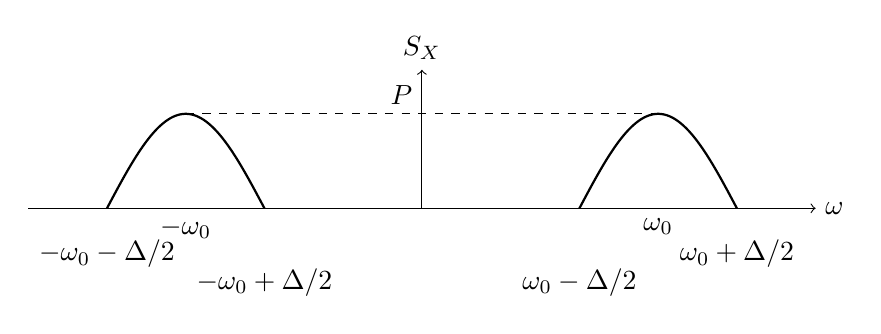
\begin{tikzpicture}[x=1cm,y=.8cm]
\draw[->](-5,0)--(5,0)node[right]{$\omega$};\draw[->](0,0)--(0,2.2)node[above]{$S_X$};
\draw[thick,domain=-1:1,samples=80]plot({-3+\x},{1.5*cos(90*\x)});
\draw[thick,domain=-1:1,samples=80]plot({3+\x},{1.5*cos(90*\x)});
\draw[dashed](-3,1.5)--(3,1.5);\node[above left]at(0,1.5){$P$};
\node[below]at(-3,0){$-\omega_0$};\node[below]at(3,0){$\omega_0$};
\node[below]at(-4,-.35){$-\omega_0-\Delta/2$};\node[below]at(-2,-.8){$-\omega_0+\Delta/2$};
\node[below]at(2,-.8){$\omega_0-\Delta/2$};\node[below]at(4,-.35){$\omega_0+\Delta/2$};
\end{tikzpicture}\end{center}
正频瓣作变量替换$\nu=\omega-\omega_0$：
\[\int_{-\Delta/2}^{\Delta/2}P\cos(\pi\nu/\Delta)d\nu=\frac{2P\Delta}\pi.\]
负频瓣面积相同，总面积$4P\Delta/\pi$。故
\[\boxed{\E X^2=\frac1{2\pi}\frac{4P\Delta}\pi=\frac{2P\Delta}{\pi^2}},\qquad
\boxed{\Var(X)=\frac{2P\Delta}{\pi^2}}.\]
最后一个等号使用题给零均值。高度$P$不是总功率，且这里频率单位为rad/s，不能漏掉$1/(2\pi)$。

\qtitle{解答 20：白噪声与有限带宽}{第7天}
{\small\color{accentred}Original exercise; tools used in 202104 Q2 and recent RC-noise questions}\par{\small\color{muted}教材小节：3.3.2 / 3.4.2 / 3.5.1}\par\smallskip\step{1. 先对有限带宽作普通反变换。}
\[\begin{aligned}R_{N_B}(\tau)&=\frac1{2\pi}\frac{N_0}{2}\int_{-B}^{B}e^{j\omega\tau}\,d\omega\\
&=\boxed{\frac{N_0\sin(B\tau)}{2\pi\tau}}.
\end{aligned}\]
在$\tau=0$取连续极限，得
\[\boxed{P_{N_B}=R_{N_B}(0)=\frac{N_0B}{2\pi}}.\]
\step{2. 理想极限只在广义函数意义成立。}
$B\to\infty$时，频域常量$N_0/2$的逆变换为$(N_0/2)\delta(\tau)$；功率则随$B$线性发散，不存在有限的瞬时方差。不能把广义函数相关在0点当作普通函数代值。
\step{3. 白与高斯是不同层次的描述。}
白描述二阶谱平坦，不决定全部概率分布，因此不自动意味着高斯。离散时间独立公平符号就是非高斯白序列；连续时间也可用对称带符号的Poisson冲激随机测度构造非高斯广义白噪声，其二阶相关为常数乘$\delta$。
教材3.1的模型却有有限边缘方差2，相关是$2\mathbf1_{\{\tau=0\}}$，不是Dirac脉冲；它不均方连续，不能与此处理想白噪声互换。

\qtitle{解答 21：两处原题模型冲突辨析}{第7天}
{\small\color{accentred}Original diagnostic based on 202312 Q1 and 202512 Q2(c)}\par{\small\color{muted}教材小节：3.1.1 / 3.3.2 / 3.4.2}\par\smallskip\step{1. 202312的谱积分发散。}
\[\frac{\omega^2}{\omega^2+16}=1-\frac{16}{\omega^2+16},\]
因此形式逆变换为
\[\boxed{R_Y(\tau)=\delta(\tau)-2e^{-4|\tau|}}.\]
谱在无穷远趋于1，故$\int S_Yd\omega=\infty$，不能对应普通有限方差WSS过程。该谱本身非负，可作广义平稳噪声的谱；此时$\delta$是分布，$\delta(0)$不是有限均方值。
\step{2. 202512的非零均值与给定相关不相容。}
若$m_A\ne0$，令$\overline A_T=T^{-1}\int_0^T A(t)dt$。连续的$R_A=e^{-|\tau|}$保证均方积分可定义，而
\[m_A^2\le\E\overline A_T^2
\le\frac1{T^2}\int_0^T\!\int_0^T e^{-|t-s|}\,ds\,dt\le\frac2T\longrightarrow0.\]
这强迫$m_A=0$，与原题冲突。这里不是仅凭相关衰减就擅自套用“极限等于均值平方”，而是给出可核验的不等式证明。
\step{3. 把修改写明。}
第一题可明确采用广义噪声解释，或把谱改为可积的非负谱，例如解答6使用的$8/(\omega^2+4)$。第二题可将给定指数解释为\textbf{协方差}$C_A$，并改写$R_A=m_A^2+e^{-|\tau|}$；另一选择是明确改设$m_A=0$。这都是额外解释或改编，不应声称原卷已经给出了这些条件。

\end{document}
